\subsection{SFERA utökat}
Genom att studera SFERA-standardens dataupsättning och lokförarnas kommunikations- och informationsbehov har de kunnat jämföras med varandra.
De överlapp som finns argumenterar för att dessa delar från lokförarnas behov täcks upp av SFERA\@.
För de delar i intervjuerna som uppdagats rörande lokförarnas nämnda behov men som inte täcks av SFERA har en utökning av SFERA tagits fram.
En illustration av detta ges i figur~\ref{fig:sferabehov}.
\begin{figure}[hbt!]
    \centering
    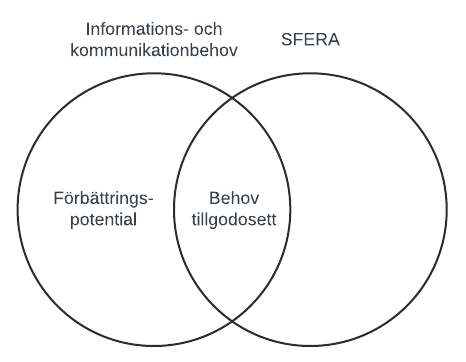
\includegraphics[width=0.8\textwidth]
    {sferabehov}
    \caption{Venndiagram som illustrerar förbättringspotential utifrån jämförelsen mellan datainsamlingsresultat och SFERA:s datauppsättning. Egen framställning.}
    \label{fig:sferabehov}
\end{figure}
\subsubsection{TMS till C-DAS-OB}
Följande förbättringsförslag ges som går utöver SFERA-protokollet för kommunikation från tågklarerare till lokförare.
\paragraph{Journey package}
Ett JP består idag av train characteristics (data om fordon), en lista över segment profile:r (data om aktuell(a) bana/banors egenskaper) samt avgångs- och ankomsttider för dessa, tillfälliga begränsningar (för exempelvis pådrag).
För att bättre möta lokförarnas behov inkluderas utöver nämn data försenings- eller omplaneringsorsak(er), avsändare av JP - vilken bandel och driftledningscentral meddelandet kommer från samt telefonnummer till denne.
Försenings- och omplaneringsinformation efterfrågas uttryckligen av förarna under intervjusessioner.
Att exempelvis veta var ett tåg ska gå om ett annat eller gå in på sidan för att släppa förbi ett tåg är ett gynnsamt sätt att bygga förtroende sett till respondenternas utsagor.
\paragraph{Blankettförberedelse}
Före muntlig ordergivning måste blanketter förberedas som lokföraren är ålagd att medtaga under tågfärd.
Ordergivning genom diktamen sker genom att lokföraren upprepar vad tågklareraren säger samtidigt som denne noterar på en blankett vilken information som tas emot.
Om tågklareraren enkelt kan uppmana en eller fler lokförare i ett område att förbereda en specifik blankett för ordergivning kan många korta samtal potentiellt sett sparas in.
Därför läggs en typ av meddelanden till i SFERA-protokollet som ska skickas från TMS via TS-servrar till C-DAS-OB när en fjärrtågklarerare vill uppmana lokförare att förbereda en specifik blankett.
\paragraph{Kontaktuppgifter}
Att veta vilket telefonnummer som går till aktuellt driftledningsområde kan vara fördelaktigt att ha lättillgängligt.
I synnerhet vid körning utomlands där det kan vara svårare att snabbt hitta rätt information.
Därför kompletteras datauppsättningen för segment profile med telefonnummer till aktuell bandels tågklarerare.
\paragraph{Trafikstörningar}
Idag kan information om trafikstörningar gå en lång omväg från en driftledningscentral innan den når lokföraren.
Om lokföraren får information direkt från ursprungskällan med plats, tid, påverkan och prognos för trafikstörningar kan information istället ges snabbt till kunder.
Ett TMS många tåg inom ett avgränsat område.
Denna funktionalitet införs därför som en ny form av meddelande.
\paragraph{Context awareness}
GPS-position av tåg tillhandahålls ett TMS som därför borde kunna återge kringliggande tågs GPS-position för ett särskilt tåg.
Att öka lokförarnas situationsmedvetenhet har pekats ut både i litteraturstudie och intervjuer som en viktig informationspunkt.
Därför kompletteras SFERA med information från IM till RU om GPS-positioner av tåg i ett enskilt tågs omgivning.
\subsubsection{C-DAS-OB till TMS}
